\documentclass[12pt]{article}
\usepackage[a4paper, total={7in, 10in}]{geometry}
\usepackage{amsmath}
\usepackage{graphicx}

\title{Analytic Geometry (Part 2) Lesson\vspace{-3mm}}
\author{2018-2019 SLSS Math Club\vspace{-5mm}}
\date{November 7, 2018\vspace{-5mm}}

\begin{document}
\maketitle
\section{Conic Sections}
A conic section (or simply conic) is a curve obtained as the intersection of the surface of a cone with a plane. The four types of conic sections are the circle, the ellipse, the parabola, and the hyperbola. \vspace{-3mm}

\begin{center}
    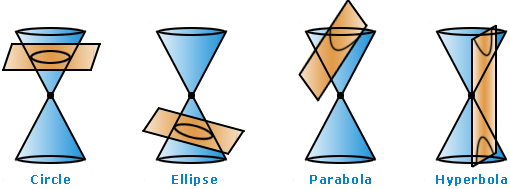
\includegraphics[scale = 1]{Graphics/Week_5/conic_sections.png}
\end{center}

\section{Eccentricity}
Eccentricity, denoted $e$ or $\epsilon$, is a variable assosiated with every conic section. It can be thought of as a measure of how much the conic section deviates from being circular. \vspace{-3mm}

\section{Curves}
\subsection{Circle}
\subsubsection{General Equation}
\begin{equation*}
    (x - h)^2 + (y - k)^2 = r^2
\end{equation*}
\begin{itemize}
    \item $h$ is the $x$ component of the circle's center
    \item $k$ is the $y$ component of the circle's center
    \item $r$ is the radius of the circle
\end{itemize}

\subsubsection{Eccentricity}
\begin{equation*}
    e = 0
\end{equation*}

\subsection{Ellipse}
\subsubsection{General Equation}
\begin{equation*}
    \frac{(x - h)^2}{a^2} + \frac{(y - k)^2}{b^2} = 1
\end{equation*}
\begin{itemize}
    \item $h$ is the $x$ component of the ellipse's center
    \item $k$ is the $y$ component of the ellipse's center
    \item $a$ is the horizontal radius of the ellipse
    \item $b$ is the vertical radius of the ellipse
\end{itemize}

\subsubsection{Eccentricity}
\begin{equation*}
    e = \sqrt{1 - \frac{b^2}{a^2}}
\end{equation*}

\subsection{Parabola}
\subsubsection{General Equation}
\begin{equation*}
    y = a(x - h)^2 + k
\end{equation*}
\begin{itemize}
    \item $a$ is the ``stretch-factor" of the parabola
    \item $h$ is the $x$ component of the parabola's vertx
    \item $k$ is the $y$ component of the parabola's vertex
\end{itemize}

\subsubsection{Eccentricity}
\begin{equation*}
    e = 1
\end{equation*}

\subsection{Hyperbola}
\subsubsection{General Equation}
\begin{equation*}
    \frac{(x - h)^2}{a^2} - \frac{(y - k)^2}{b^2} = 1
\end{equation*}
\begin{itemize}
    \item $h$ is the $x$ component of the hyperbola's center
    \item $k$ is the $y$ component of the hyperbola's center
    \item $a$ horizontal distance between the center and a vertex of the hyperbola
\end{itemize}

\subsubsection{Eccentricity}
\begin{equation*}
    e = \sqrt{1 + \frac{b^2}{a^2}}
\end{equation*}

\subsubsection{Asymptotes}
\begin{equation*}
    y = \pm \frac{b}{a}x
\end{equation*}
\end{document}